%% $RCSfile: using.tex,v $
%% $Revision: 1.1 $
%% $Date: 2010/04/23 01:57:05 $
%% $Author: kevin $
%%
\chapter{Literature Review}\label{C:background}
This chapter begins by providing a brief introduction of Cloud computing and the energy consumption problem in cloud data centers. Section \ref{resource_management} introduces resource management in cloud including the placement decision scenarios (Section \ref{scenarios}) and the main strategy - server consolidation (Section \ref{consolidation}).The second part (Section \ref{related_work}) gives a literature review on resource management in both container and VM-based cloud. 

% This chapter begins by providing a fundamental background to the field of Cloud computing in Section \ref{sec:background}.
% Section \ref{} discusses the resource allocation in PaaS as well as the bi-level optimization including both biologically and non-biologically
% inspired approaches; Section \ref{} delves into approaches that optimize the static placement. In addition, time-series aware problems and their approaches will be discussed; Section \ref{} discusses the issue of dynamic server consolidation and genetic programming; Section \ref{} covers approaches of scalability; Finally, Section \ref{} presents a summary of the important points identified in this review, alongside a discussion of the limitations of existing approaches.


\section{Cloud Computing and Energy Efficiency Problem}
\label{sec:background}


\bx{Cloud computing is a computing model that offers a network of servers to their clients in a on-demand fashion.} From NIST's definition \cite{Mell:2011jj}, \textit{"cloud computing is a model for enabling ubiquitous, convenient, on-demand network access to a shared pool of configurable computing resources (e.g., networks, servers, storage, applications and services) that can be rapidly provisioned and released with minimal management effort or service provider interaction."} Hence, Cloud computing has major functionalities for providing facilities to cloud users.

\begin{figure}
	\centering
	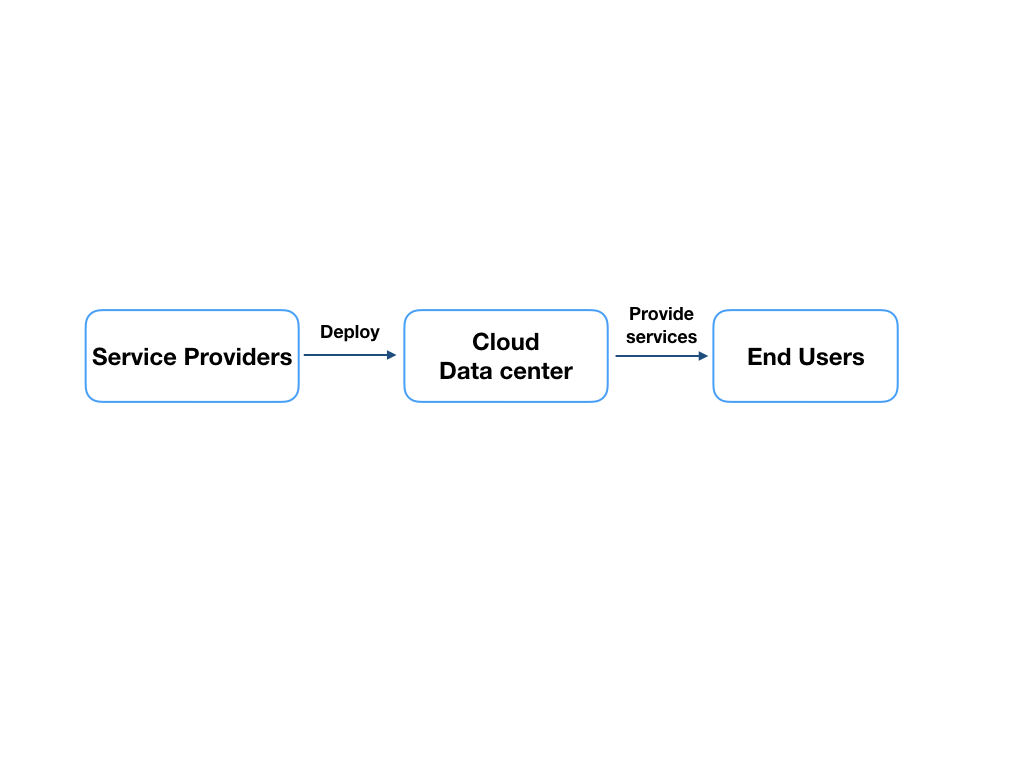
\includegraphics[width=0.6\textwidth]{pics/stakeholders.png}
	\caption{Stakeholders of Cloud computing \cite{Jennings:2015ht}}
	\label{fig:stakeholders}
\end{figure}

\bx{To give an example of how Cloud computing works (see Figure \ref{fig:stakeholders}), consider the case:} a \emph{Cloud provider} builds a data center containing thousands of servers. These servers connect with a network. 
To use these remote servers, \emph{Cloud user} (e.g an application provider), can deploy and access their applications (e.g Endnote, Google Drive and etc.) in these servers from anywhere in the world. Once the applications start serving, \emph{End users} can use them without installing on their local computers. Cloud providers charge fees from Cloud users for infrastructure. Cloud users charge fees from End users for using applications. \tran{Therefore, from cloud providers' perspective, both accommodating more applications and reducing energy consumption lead to the increase of profit.}

\bx{The major expense of a cloud provider is energy consumption \cite{Kaplan:up01fR-k} and physical machines (PMs) (e.g servers) contribute to a majority of the energy.} As shown in Figure \ref{fig:consumption}, both the cooling system and physical machines (PMs) account for 40\% of energy. However, PMs' energy efficiency are low on average  \cite{Hameed:2016cmb}.
The reason for low energy efficiency is the disproportion between the utilization of PMs and the energy consumption of PMs. \howto{For example, when CPU utilization of a PM is 15\%, the energy consumption of the PM is 70\% of its peak time.} Therefore, 
cloud providers can reduce the energy consumption by improving the utilization of PMs.


\tran{In order to solve the low energy efficiency caused by low utilization of PMs, cloud providers use a resource management system to manage the applications.}

\begin{figure}
	\centering
		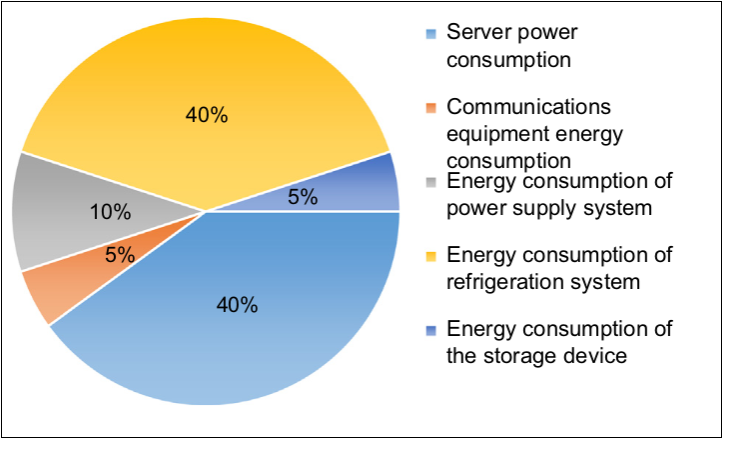
\includegraphics[width=0.35\textwidth]{pics/energyConsumption.png}
		\caption{Energy consumption distribution of data centers \cite{Rong:2016js}}
		\label{fig:consumption}

\end{figure} 

\section{Cloud Resource Management}
\label{sec:resource_management}
\bx{Cloud resource management is a process of allocating computation resources (e.g CPU and memory) to Cloud users to run their applications. Meanwhile, resource management aims to achieve low energy consumption in cloud} \cite{Jennings:2015ht}.

Resource management applies two types of virtualization: virtual machine (VM) and container on four management steps (see Section \ref{sec:statement}): collecting PMs' utilization data, analyzing available PMs, deciding the placement of applications, and executing the placement. Furthermore, in the third step of placement decision, resource management has three common scenarios: initial placement, periodic placement, and dynamic placement. Resource management uses distinct server consolidation strategies on these placement scenarios based on different virtualiazation technologies to achieve energy efficiency. 

This section will first introduce and compare two types of virtualization: VM-based and container-based and then illustrate 
three placement decision scenarios. 

\subsection{Virtualization Technologies}
\label{sec:virtualization}

\bx{Resource management uses virtualization technologies \cite{Uhlig:2005do} to achieve a finer granularity management than the traditional way.} In comparison with traditional management -- allocating an application to a PM -- virtualized management partitions PM's resources (e.g. CPU, memory and disk) into several independent units and allocates applications into these units. 
The most common units are virtual machines (VMs) and containers.

Virtualization technology rooted back in the 1960s' was originally invented to enable isolated software testing. Because VMs can provide good isolation for applications running without interfering with each other \cite{Somani:2009ho}. Soon, people realized that virtualization can improve the utilization of hardware resources: with each application deployed in a VM, a PM can run multiple applications. 

The next two sections illustrate two classes of virtualization (see Figure \ref{fig:comparison}): VM-based and container-based virtualization and then compares the two virtualizations.

\begin{figure}
	\centering
	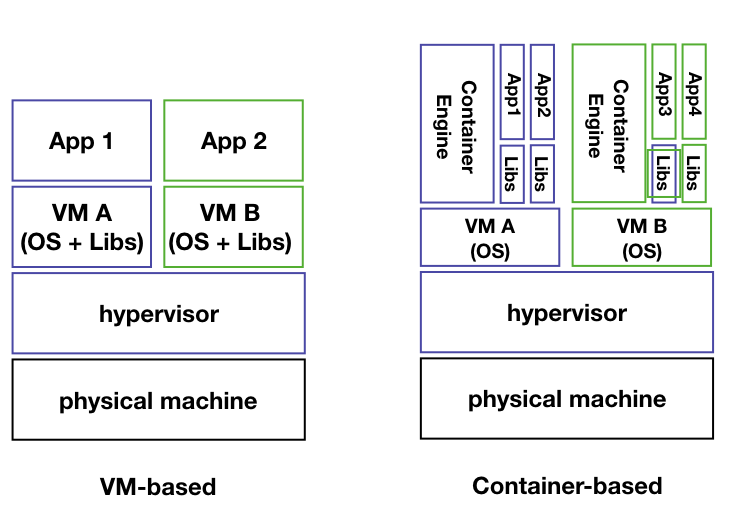
\includegraphics[width=0.7\textwidth]{pics/comparison.png}
	\caption{A comparison between VM-based and Container-based virtualization \cite{Piraghaj:2016bw}}
	\label{fig:comparison}
\end{figure}

\subsubsection{VM-based Virtualization} 

\bx{A VM-based virtualization has three-layers of structure: PM-Hypervisor-VM (see Figure \ref{fig:comparison} left-hand side).} 
The hypervisor or the virtual machine monitor (VMM) is a software layer on top of PM. A hypervisor arbitrates accesses to the PM's resources so that VMs can share resources on the PM. Some implementations of VM-based hypervisors such as Xen \cite{Barham:2003cj}, KVM \cite{Kivity:2007wu}, and VMware ESX \cite{Waldspurger:2002db} dominate this field in recent years. On of top of hypervisor, \textbf{VMs} are the fundamental resource management units. A VM allows independent Operating System (OS) to run on it.  

In addition, hypervisors support dynamic migration techniques (e.g pre-copy \cite{Clark:2005ud} and post-copy \cite{Hines:2009fv}) that can move VMs from one PM to another. Therefore, resource management can improve the utilization of a PM by migrating VMs to that PM.


\subsubsection{Container-based Virtualization} 

\begin{figure}
	\centering
	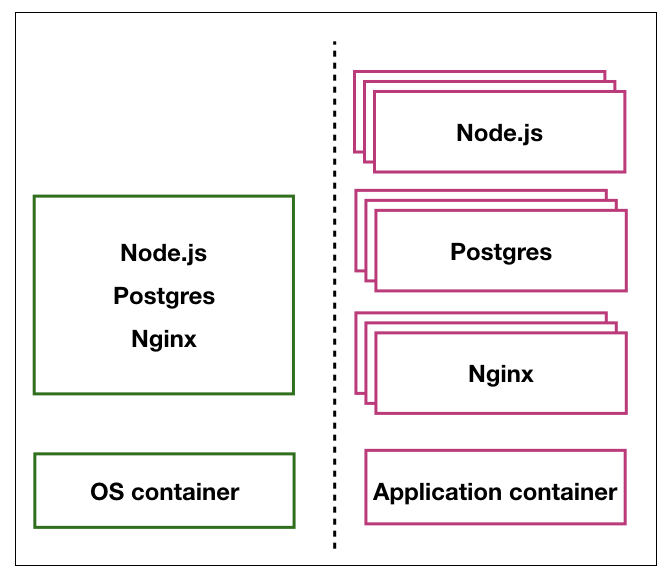
\includegraphics[width=0.4\textwidth]{pics/container_OS_APP.png}
	\caption{A comparison between OS container and Application container \cite{Piraghaj:gb}}
	\label{fig:comparison_container}
\end{figure}

\bx{A Container-based virtualization has four-layers of structure: PM-Hypervisor-VM-Container (see Figure \ref{fig:comparison} right-hand side).} Container-based virtualization is also addressed as operating-system-level virtualization because containers run on top of VMs. Specifically, container-based virtuliazation includes two classes: OS container and application container \cite{Piraghaj:gb}. 

\bx{OS containers (Figure \ref{fig:comparison_container} left-hand side) have a one-on-one relationship with VM.}
Multiple applications run inside an OS container. Three implementations of OS-level of containers: OpenVZ, Google's control groups, and namespace \cite{Rosen:2013wt} are widely used in Google and Facebook.

\bx{Application containers (Figure \ref{fig:comparison_container} right-hand side) have a many-to-one relationship with VM.} A single application runs on an application container. Major implementations such as Docker, Rocket and Kubernetes \cite{Bernstein:2014ur} are very popular in the software industry. 

\bx{In comparison with OS container, an application container is much more flexible because each container has its separated environment (e.g. libraries) for applications.} Furthermore, application containers provide a finer granularity of resource management by enabling an application level of operations including deployment, scaling, and migration.  

Notice that, in the following content, we use ``container'' to represent ``application container''. 
We do not discuss Os container because it is very similar to a VM.


\subsubsection{Comparison between Container-based and VM-based Virtualization} 
\label{sec:comparison_container_vm}
\bx{This section summarizes three disadvantages of VM-based virtualization in terms of energy efficiency and shows how container-based can overcome these disadvantages based on several research~\cite{Felter:2015ki, Xavier:2013fy, Dua:2014bw}.}  


Some main disadvantages in VM-based virtualization are listed as follows:
\begin{itemize}
	\item Resource over-provisioning \\
	\bx{Cloud users tend to reserve more resources for ensuring the Quality of Service at peak hours \cite{Chaisiri:2012cva}} The over reserved resources lead to low resource utilization. Cloud users do not completely rely on auto-scaling because auto-scaling is more expensive than reservation. However, the peak hours only account for a short period, therefore, for most of the time, resources are wasted.

	\item Unbalanced usage of resources \\
	\bx{Specific applications consume unbalanced resources.} The unbalanced resources lead to a vast amount of resource wastage \cite{Tomas:2013iv}. For example, computation intensive tasks consume much more CPU than RAM; a fixed type of VM provides much more RAM than it needs. Because the tasks use too much CPU, they prevent other tasks from co-allocating. This also causes wastage.

	\item Heavy overhead of VM hypervisors and redundant operating systems (OSs) \\
	\bx{Heavy overhead of  hypervisors and redundant OSs running in the PM also causes huge resource wastage.} Traditional VMs provide a complete independent environment that includes its own OS and libraries for deploying software. However, as most applications only require a general OS such as Windows or Linux, multiple duplicate OSs running in the system is a waste of resource.
\end{itemize}


Some key characteristics of containers can help overcome the above disadvantages of VMs.

The following two characteristics can overcome the heavy overhead of VM hypervisors and reduce the redundant OSs.
\begin{itemize}
	\item Container-based virtualization has lightweight management that generates much less overhead than a VM hypervisor. 
	\item Container-based virtualization shares OSs. Therefore, fewer VMs reduce overheads of multiple OSs.

	\item Container-based virtualization naturally supports vertical scaling while VM-based virtualization does not. Vertical scaling means a container can dynamically adjust its resources under the host's resource constraint. This feature offers a fine granularity management of resources. 

\end{itemize}

	Vertical scaling can overcome the resource over-provisioning by dynamically adjusting the size of containers. Furthermore, the size of container reflects the requirement of the application. We can achieve a balanced usage of resources by using appropriate placement algorithm.


\bx{In summary, container-based virtualization has the potential to further improve the energy efficiency than VM-based virtualization.} No matter which virtualization technology is used, the cloud often deals with three placement decision scenarios. 




\subsection{Placement Decision Scenarios}
\label{sec:scenarios}

\bx{Three placement decision scenarios \cite{Svard:2015ic, Mishra:2012kx}: initial placement of applications, periodic placement of applications, and dynamic placement of applications (see Figure \ref{fig:management}).}

\begin{figure}
	\centering
	\begin{subfigure}[b]{0.9\textwidth}
		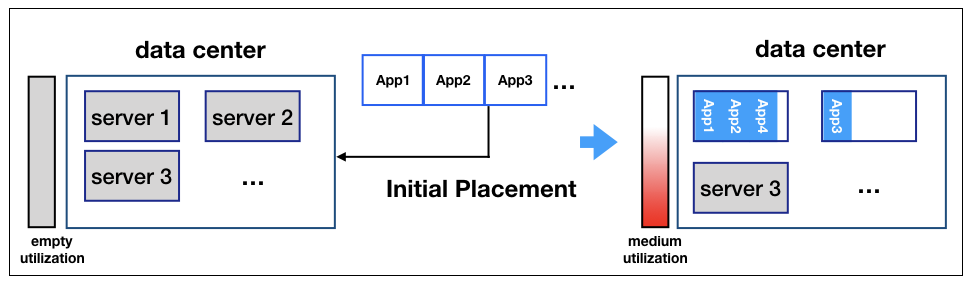
\includegraphics[width=\textwidth]{pics/initial_placement.png}
		\caption{Initial placement of applications}
	\end{subfigure}
	\begin{subfigure}[b]{0.9\textwidth}
		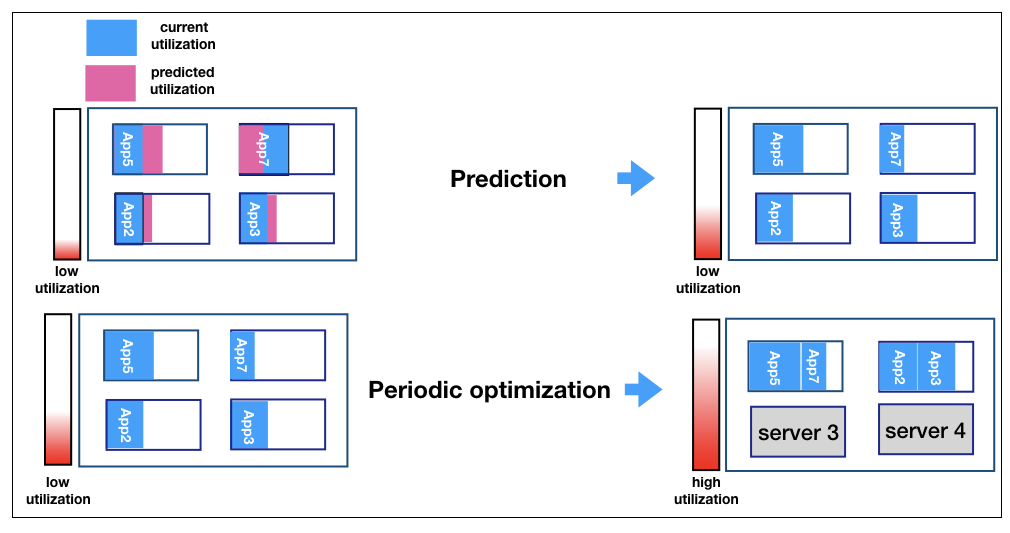
\includegraphics[width=\textwidth]{pics/periodic_optimization.png}
	\caption{Periodic placement of applications}
	\end{subfigure}
	\begin{subfigure}[b]{0.9\textwidth}
		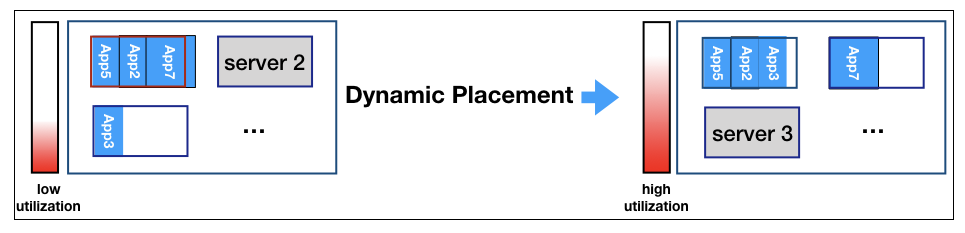
\includegraphics[width=\textwidth]{pics/dynamic_placement.png}
	\caption{Dynamic placement of applications}
	\end{subfigure}
	\caption{Three scenarios of placement decision}
	\label{fig:management}
\end{figure}

\paragraph{Initial Placement of Applications} is applied when new applications arrived. The task is to place applications into a set of PMs \cite{Mishra:2012kx} so that PMs satisfy all applications' resource demands and minimize the energy consumption.



\paragraph{Periodic Placement of Applications} is applied periodically to adjust the current placement of applications. The task is to re-place the current applications so that resource management minimizes the energy consumption and minimizes the cost of migration.

\paragraph{Dynamic Placement of Applications} is applied in two scenarios \cite{Mishra:2012kx}: Overloading and underloading. Overloading is a scenario where the total demands of applications in a PM are higher than the PM's resources. Therefore, the PM causes a degradation in one or more applications' performance. Underloading is a scenario where the PM is running in low utilization. In both scenarios, resource management moves the applications from one PM to another PMs in an on-line fashion~\cite{Borodin:2cY4439E}.

Next section will discuss general server consolidation strategies.

\subsection{Server Consolidation Strategy}
\label{consolidation}

\begin{figure}
	\centering
	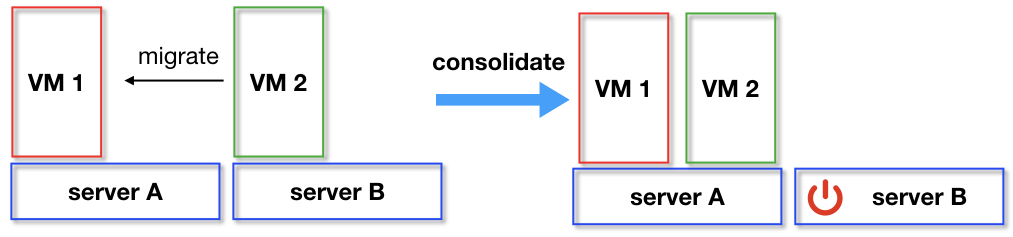
\includegraphics[width=0.7\textwidth]{pics/consolidate.png}
	\caption{A Server Consolidation example: Initially, each PM runs an application wrapped with a VM in a low resource utilization state. After the consolidation, both VMs are running on PM A, so that PM B is turned off to save energy \cite{Barroso:2007jt}.}
	\label{fig:consolidation}
\end{figure}


\bx{Server consolidation is a resource management strategy that aims to improve the utilization of PMs and reduce the energy consumption.} We use VM-based virtualization as an example: a general step of server consolidation is shown in Figure \ref{fig:consolidation}, a number of VMs is migrated to fewer number of PMs. Resource management applies Server consolidation to solve 
the low utilization of PMs called PM sprawl~\cite{Khanna:2006vq}.

% \subsubsubsection{Model}
\begin{figure}
	\centering
	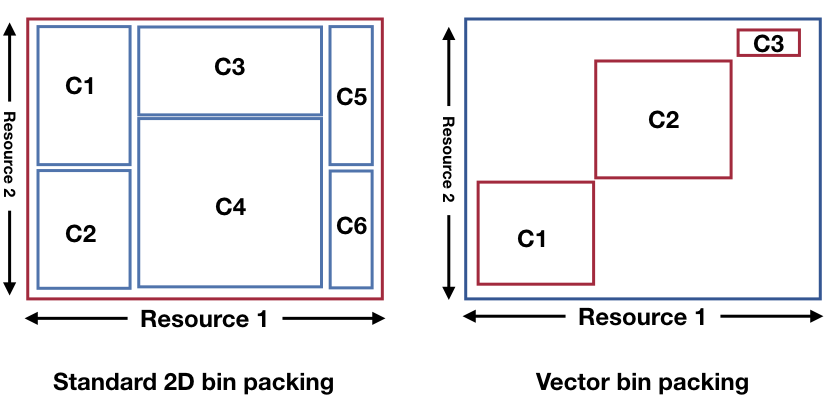
\includegraphics[width=0.6\textwidth]{pics/bin_packing_problem.png}
	\caption{A comparison between standard bin packing and vector bin packing}
	\label{fig:bin_packing_problem}
\end{figure}

\subsubsection{Types of Server Consolidation}

% Three major benefits of virtualization make it be the first choice for web-based application consolidation: No reliance on hardware, easy to provision and live migration.

\bx{Server consolidation can be done in two ways: Static and dynamic \cite{Xiao:2015ik, Verma:2009wi} based on different scenarios.} Initial placement and periodic placement involve large number of variables, therefore, they are very time-consuming job and often conducted in an off-line fashion. Dynamic placement requires a fast decision-making to place one application to PMs. Thus, resource management uses a dynamic server consolidation strategy to handle the scenario. 



\section{Evolutionary Computation}
\bx{Evolutionary Computation (EC) algorithms are artificial intelligent algorithms that are inspired by biological mechanisms of evolution, social interactions and swarm intelligence.} They are famous for strong search ability because they have several distinguished characteristics such as the use of a population-based search and the ability of avoiding local optima. EC algorithms have been applied successfully to solve a variety of real-world problems \cite{Engelbrecht:dm}, especially, combinatorial optimization problems.

% A common process of EC algorithms is as follows. Initially, the population are randomly generated in the search space. During the evolution process, the population
% explores according to the evaluation of a or multiple predefined fitness functions. At the end of the evolution, the individual with the best fitness value is selected as the output.

\bx{Researchers have proposed a variety of EC algorithms \cite{Yao2006} to solve optimization problems.} The majority of current EC algorithms descends from three major approaches: \emph{genetic algorithms (GAs)}, \emph{particle swarm optimization (PSO)} and \emph{genetic programming (GP)}. 


This section will first introduces these three important EC algorithms that we would like to use in our future work. Then, we will review a number of EC algorithms that are used in combinatorial optimization problems. From these problems, we will conclude some of the advantages of using EC algorithms in solving resource allocation problem in clouds.

\subsection{Genetic Algorithms (GAs)}
% GA \cite{Holland:1962fy} was introduced by Holland. Since then, a large number of applications \cite{DeJong:1992vk, DeJong:1992ws} have applied GA  as their search mechanism. 
\bx{GA is a population-based search algorithm \cite{Vose:1993iu}.} In GA, the solution of a problem is coded as a vector of numbers called chromosome or individual. A GA searches for the best solution by iteratively changing the values in the chromosome. 

\bx{We describe a general GA procedure as follows.} In the beginning, a population of chromosomes which represents the solutions of the problem are often represented as a fixed length string. Each entry or bit can be continuous, discrete or even alphabets depending on the problem.  The evolution often starts from randomly generated population followed by an iterative process called generation.  In each generation, the fitness value of chromosomes is evaluated according to a defined fitness function.  Then, genetic operators such as mutation and crossover are applied on the solutions so that they are modified. As a search mechanism, these operators move solutions to explore the search space. New generations of solutions are then evaluated by the fitness function.  This evolutionary procedure ends when a predefined generation number or a satisfactory level of fitness has been reached.

\begin{figure}
	\centering
	\begin{subfigure}[b]{0.44\textwidth}
		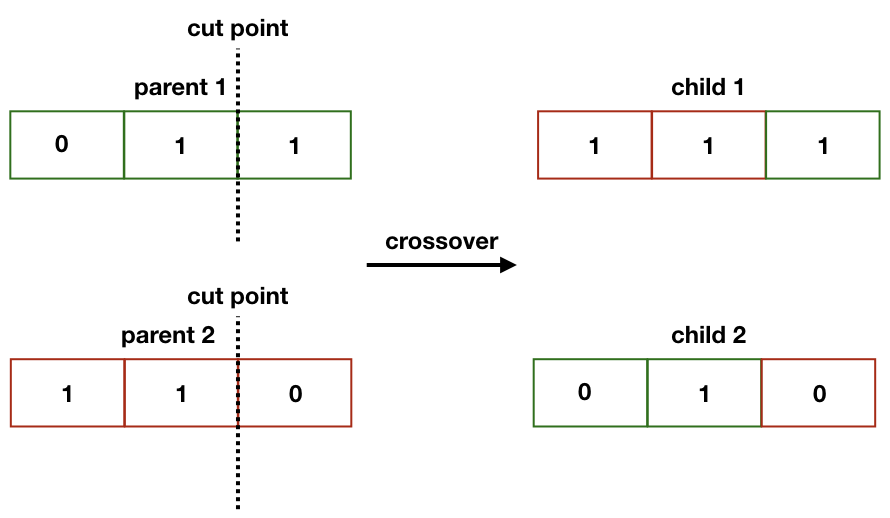
\includegraphics[width=\textwidth]{pics/crossover.png}
	\caption{Crossover}
	\end{subfigure}
	\begin{subfigure}[b]{0.44\textwidth}
		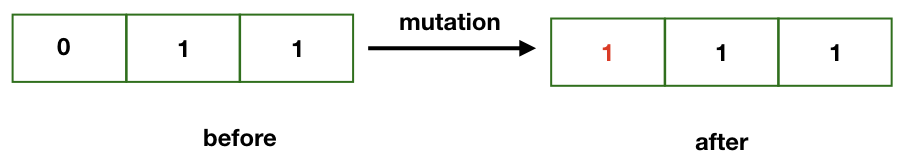
\includegraphics[width=\textwidth]{pics/mutation.png}
	\caption{Mutation}
	\end{subfigure}
	\label{fig:operators}
\end{figure}

\bx{GA-based algorithms are suitable for off-line combinatorial optimization problems.} Different from traditional algorithm such as Integer linear programming (ILP) technique, a GA-based algorithm bypasses the complicated procedure of tunning parameters by searching through the solution space of a problem. Although a GA-based algorithm does not guarantee a global optima solution, a GA-based algorithm normally can provide a near-optima solution within feasible amount of time. Although a GA-based algorithm spends less time than an ILP, it still takes too long time than an on-line problem requires. Therefore, we will consider use a GA-based algorithm in the first and second objectives: initial placement of applications and periodic placement of applications. 

GA-based algorithms have been applied to a variety of combinatorial optimization problems such as the assembly line balancing problem \cite{Anderson:1994io}, scheduling in Grid computing \cite{Zomaya:2005bb} and resource allocation problem in clouds \cite{Wilcox:2011ea}. Specifically, we will discuss the literature that applied GA-based algorithms in the server consolidation strategies in Section \ref{sec:related_work}. 

Next section will introduce another popular algorithm: particle swarm optimization (PSO). 


% Evolutionary programming, introduced by Fogel \cite{Fogel:1962wv}, was originally designed to generate artificial intelligence. 
% Evolutionary strategies as developed by Rechenberg \cite{Rechenberg:a_aZDNtZ} and Schwefel \cite{Schwefel:Nd2pzTwG}, were initially designed with the goal of solving difficult discrete
% and continuous, mainly experimental, parameter optimization problems \cite{Klockgether:1970tw}. 

\subsection{Particle Swarm Optimization (PSO)}
\bx{PSO is a meta-heuristic algorithm inspired by the social behavior of birds \cite{Eberhart:1995tj}.} In PSO, each individual -- a particle -- searches the solution space. The underlying phenomenon of PSO is to use the collective knowledge to find the optimal solution.

\bx{We describe the procedure of PSO as follows.} At the initial state, each particle has a random initial position in the search space that is represented by a vector $\vec{x}_i = (x_{i1}, x_{i2}, \dots, x_{iD})$, where \emph{D} is the dimension of the search space. A particle has a velocity as $\vec{v}_i = (v_{i1}, v_{i2}, \dots, v_{iD})$. The velocity is limited by a threshold $v_{\max}$ so that for any $i$ and $d$, $v_{id} \in [-v_{\max}, v_{\max}]$. During the search process, each particle maintains a record of its best position so far, called the \emph{personal best} ($pbest$). The best position among all the personal best positions of its neighbors is the \emph{global best} ($gbest$). The position and velocity of each particle are updated according to the following equations:
\begin{equation}
\label{eq:updatePosition}
x^{t+1}_{id} = x^{t}_{id} + v^{t+1}_{id},
\end{equation}

\begin{equation}
\label{eq:updateVelocity}
v^{t+1}_{id} = w \cdot v^{t}_{id} + c_1 \cdot r_{1i} \cdot (p_{id} - x^t_{id}) + c_2 \cdot r_{2i} \cdot (p_{pg} - x^i_{id}).
\end{equation}

Here, $t$ is the index of iteration. $d$ is the index of dimension. The inertia weight $w$ is used to balance the local search and global search abilities. The parameters $c_1$ and $c_2$ are the acceleration constants. $r_{1i}$ and $r_{2i}$ are random constants following the uniform distribution in the interval $[0, 1]$. $p_{id}$ and $p_{gd}$ denote the values of $pbest$ and $gbest$ in the $d^{th}$ dimension of the $i^{th}$ particle.

\bx{PSO-based algorithms are also suitable for combinatorial optimization problems.} Although PSO was originally developed for optimizing problems with continuous representations (e.g. real-value), the recent development of PSO support the discrete problem as well. Specifically, the binary PSO \cite{Kennedy:1997hd} is designed for binary problems; the discrete PSO \cite{Liao:2007dl} is designed for scheduling problems; and a Combinatorial PSO \cite{Jarboui:2007in} is developed for problems with integer representation. In the literature, PSO-based algorithms have also been applied for resource allocation problem \cite{Xiong:2014jq}. We will discuss these approaches in Section \ref{sec:related_work}.


\bx{Compared with GA-based algorithms, PSO-based algorithms have a faster convergence speed.} However, PSO-based algorithms are more easier to be stuck at local optima for large dimensional problems than GA-based algorithms. Therefore, sometimes PSO-based algorithms can be used in dynamic problems if the number of variables is small. More often, PSO-based algorithms are applied in off-line problems like GA. Therefore, we will also consider using PSO in the first and second objectives.

Next section will introduce the genetic programming-based hyper-heuristic (GP-HH), which is suitable for dynamic problems.

\subsection{Genetic Programming-based Hyper-heuristic (GP-HH)}

Genetic programming \cite{1992gppc.book.....K} is an evolutionary computation technique, inspired by biological evolution, to automatically find 
computer programs for solving a specific task. In a GP population, each individual represents a computer program. In each generation, these programs are evaluated by a predefined fitness function, which accesses the performance of each program. Then, individuals will go through several genetic operators such as selection, crossover, and mutation. A number of top individuals will survive to the next generation while others will be discarded. The major difference between GA and GP is that each GP individual is represented as a tree with variant depth instead of a string. This representation is particular suitable for a program. For example,  a GP individual is shown in Figure \ref{fig:gp_program} which is a program x + max(y $\times$ 2, -2). The variables \{x, y\} and constraint \{-2, 2\} are called terminal of the program. The arithmetic operations \{+, $\times$, max \} are called functions in GP. A GP individual is a specific combination of elements in a terminal set and a functional set. In order to observe the relationship between a function and its subtrees, the GP programs are usually presented to human users by using the $prefix$ notation similar to a Lisp expression, for example, x + max(y $\times$ 2, -2) can be expressed as (+ (x (min ($\times$ y 2) -2 ))).

\begin{figure}
	\centering
	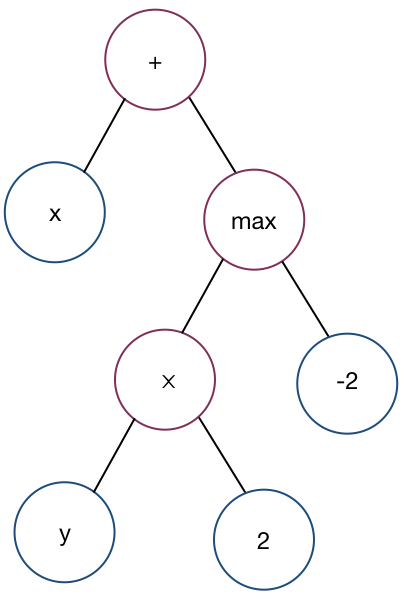
\includegraphics[width=0.3\textwidth]{pics/gp-tree.png}
	\caption{GP program that represents x + max(y $\times$ 2, -2)}
	\label{fig:gp_program}
\end{figure}


GP-based hyper-heuristics (GP-HH)  has been applied in many applications such as Job shop scheduling to evolve dispatching rules \cite{Nguyen:2014eu}. The term hyper-heuristics \cite{Cowling:2000ek} means ``heuristics to choose heuristics''.
\emph{Dispatching rule} is essentially a heuristics \cite{Panwalkar:1977fw} used in a scheduling context. 
Resource allocation problems are also in the scheduling category and they are often modeled as bin packing problems. 
GP-HH has been applied in generating heuristics for bin-packing problems \cite{Poli:2007kt,Sim:2013fe,Burke:2012gs}. These research studies have shown that GP-HH can generate excellent heuristics which have equal or better performance than human designed heuristics.

In the Cloud computing context,  Cloud resource allocation usually has extra constraints such as multi-dimensional resources, migration costs, heterogeneous PMs, etc. These constraints make the Cloud resource allocation problem much harder than original bin packing \cite{Mann:2015ua}. Therefore, traditional bin packing approaches such as First Fit Decreasing, Best Fit, etc, cannot perform well in this context.  GP-HH, therefore, is a promising technique that can be used to automatically generate heuristics under multiple constraints.

\subsection{EC Algorithms in Combinatorial Optimization}
This section will review a number of EC algorithms in two typical combinatorial optimization fields: cloud computing resource allocation and job shop scheduling. 

\paragraph{Cloud Computing Resource Allocation}
Traditional cloud computing resource allocation includes six categories \cite{Guzek:2015ds}: cloud brokering, VM placement, service placement and workflow scheduling are typically static problems; server load balancing and cloud capacity planning are dynamic problems. EC algorithms have been applied in problems in each of these categories. This section will briefly review approaches used in these problems except VM placement. We will explicitly discuss VM placement in Section \ref{sec:related_work}.

\vspace{5mm}

In cloud brokering problem, a cloud broker is an intermediary between cloud users and cloud providers. Cloud brokers estimate the resource requirements and choose resources for cloud users. The objective of cloud brokering is to minimize the cost for cloud users as well as guarantee the quality of service (QoS) of cloud users' applications.

Frey et al \cite{Frey:2013gp} propose a GA approach (CDOXploer) for finding near-optimal cloud deployment architectures and runtime reconfiguration rules for softwares. Their approach takes into account VM types, the number of VMs, and the scaling policies of VMs. CDOXplorer minimizes response times, costs, and SLA violations in order to satisfy the requirement of cloud users.  In comparison with Frey's centralized approach, Iturriaga et al \cite{6681297} propose an Evolutionary Algorithm (EA) with distributed sub-populations. In each sub-population, they applied a Simulated Annealing (SA) method to find the local optimal solution. The proposed algorithm is shown outperform than the reference list scheduling algorithm in both computation time and performance (maximizing the profit of a broker).

\vspace{5mm}

In service placement problem, cloud users would like to optimize the costs and performance (e.g QoS) of their services. Compared with cloud brokering problem, service placement less focuses on resource allocation but more focuses on the latencies between locations. Cloud users need to decide the locations of services and the number of services \cite{Guzek:2015ds}. 

Tan et al \cite{Tan2017} propose an aggregation approach with binary PSO to solve the service placement problem with two objectives: minimizing cost and minimizing the response time. They find that the single-objective algorithm can only provide one solution for each run, hence, single-objective algorithm cannot provide alternatives when cloud users do not have preferences. Therefore, they develop an NSGA-II based approach \cite{Tan2016} that uses Pareto front approach to find a set of non-dominated solutions. They conclude that multi-objective evolutionary algorithms are suitable for the service placement problem.

\vspace{5mm}

The workflow scheduling problem allocates a set of dependent services, organized as a directed acyclic graph (DAG). The objectives of workflow scheduling are minimizing makespan and cost. The major difference between workflow scheduling and service placement is the extra constraint on the order of services. Another difference is that workflow scheduling rarely considers the latency issue. Compared with cloud brokering problem, workflow scheduling problems have additional dependencies between applications.

 Tsai et al \cite{Tsai:2013fn} develop an Improved Differential EA (IDEA) to solve the multi-objective scheduling problem. They represent the solution as a permutation of subtasks. They also design a crossover operator that only changes the resource allocation of subtasks and a mutation operator that changes the task order. They compare IDEA with NSGA-II, SPEA2, and DEA in two test scenarios. The results show their approach outperforms than other EC algorithms. 

\vspace{5mm}

Capacity planning problems estimate the future load of VMs and PMs before allocating resources.
The major objectives is to optimize the QoS while minimizing the cost of users. Different from above problems, the capacity planning problem is often treated as a dynamic problem. 

Kousiouris et al \cite{Kousiouris:2013vg} propose an artificial neural (ANN) network-based framework to predict the load of a GNU Octave system. They use a GA to create the structure of ANN and the ANN is encoded using a bit-string representation. The algorithm can be trained off-line and test on-lien. Therefore, it is well-suit for a dynamic problem.

\vspace{5mm}

Similar as the capacity planning problem, server Farm Load Balancing problem is also a dynamic problem. The task is to dispatch incoming requests to a set of machines. The major objective is to satisfy the QoS (e.g. makespan) of cloud users.

Laredo et al \cite{Laredo:2014db} propose an on-line and decentralized scheduler for distributing Bag-of-task kind of workloads to heterogeneous infrastructures. Their approach mimics the behavior of sandpile. They manage cloud resources (PMs) by segmenting resources and assign each segmentation with a monitor called agent. These agents interact with their neighbors (predefined) and share their information about resources. Tasks arrive to PMs and accumulate as grains of sand. When an agent detects an unbalance between a segment of resources and its neighbors, it triggers an avalanche. They test the system with very large scale problems: 2048 PMs and 2048 tasks and achieve at least five times better in terms of makespan and throughput than a round robin algorithm.

Server Farm load balancing is very similar to another classic problem: job shop scheduling (JSS). They both dispatch a set of jobs to a set of machines except load balancing problem focus more on computing resources such as CPUs and memories. In the next section, we will introduce JSS and the EC methods applying on JSS.
\paragraph{Job Shop Scheduling}
Job shop scheduling (JSS) problems \cite{Potts:2009eb} dispatch a set of jobs to machines. A job goes through a predetermined sequence of operations in order to finish its tasks. Each machine can only process a specific operation. Therefore, we need to make intelligent decisions to schedule these jobs in order to finish processing jobs before their due dates.

JSS problems can be divided into two categories: static and dynamic. In static JSS problems, all properties of jobs and machines are known in advance. In dynamic JSS problems, properties of jobs are unknown.  

The state-of-the-art approaches for static JSS problems use meta-heuristics. Examples of meta-heuristics approaches to JSS include Tabu search \cite{AmaralArmentano:2000dk}, GA \cite{Zhou:2009dq} and etc. These meta-heuristics can handle large JSS problem instances effectively. 

Dynamic JSS problems often apply small heuristics such as dispatching rules \cite{Branke:2016wy} because dispatching rules have short reaction times and can quickly deal with unforeseen changes in an on-line event. For example, a SPT (shortest processing time) selects the job with the shortest processing time waiting at the available machine. Apart from simple dispatching rules, composite dispatching rules (CDRs) \cite{Jayamohan:2004kq} combine several simple dispatching rules to achieve higher performance. 

However, it is difficult to design dispatching rules for dynamic JSS problems. This is because, first, no single dispatching rule is more effective than others for all JSS problems. Second, a real-world dynamic JSS problem is changing over time, e.g. machines are added and removed. Therefore, designing dispatching rules often requires domain knowledge. 

To design dispatching rules more effectively, researchers use a hyper-heuristic technique to automatically generate dispatching rules. Specifically, a great number of hyper-heuristic approaches to JSS problem uses Genetic Programming (GP) technique called GP hyper-heuristic (GP-HH). GP-HH represents dispatching rules with a tree-based representation and these dispatching rules can be interpreted as priority-based dispatching rules. GP-HH approaches generally outperform manually designed dispatching rules for both static and dynamic JSS problems \cite{Branke:2016wy}. 

In comparison between the dynamic JSS problem and the dynamic placement of applications, they share many similarities. First of all, they are both on-line problems that require a fast reaction. Second, they both dispatch jobs to machines. The differences are the dynamic JSS problem normally does not care the amount of resources that a job consumes. The dynamic placement not only considers the resource requirement of jobs but also the remaining of resources in Physical machines (PMs). Another difference is that the jobs in dynamic JSS go through a route of machines while the jobs in dynamic placement stay at one machine.

The similarities inspire us to apply GP-HH approach on the dynamic placement of applications problem.

\vspace{5mm}


In conclusion, EC-based algorithms have been widely used in resource allocation problems in cloud for both static problems and dynamic problems. Specifically, meta-heuristics such as GA and PSO are more suitable for static problems and hyper-heuristics such as GP are suitable for dynamic problems. 
We conclude several advantages of EC approaches. First, EC-based algorithms rely on searching in the solution space, which bypass the complexity of finding the exact mathematical approach. Second, EC-based algorithms are population-based algorithms, which can find near-optimal solutions within a feasible amount of time.
Next section will provide the literature of traditional approaches and EC-based approaches on server consolidation strategies in terms of two virtualization: container and VM. 


\section{Related Work}
\label{sec:related_work}
Related work discusses the server consolidation strategy and the studies of consolidation strategies on three placement decision scenarios: initial placement, periodic placement, and dynamic placement. 


\subsection{Initial Placement of Applications}
\label{sec:initial}

This section first discusses server consolidation strategies on container-based virtualization and VM-based virtualization.

\subsubsection{Container-based Initial Placement of Applications}
\label{container-based-placement}
This section will discuss existing approaches for container-based initial placement. Then, we will describe a potentially way of modeling energy consumption in container-based virtualization: a bilevel model. Last, we will illustrate a number of algorithms to solve bilevel optimization problems. 


\paragraph{Existing Approaches}

\bx{We discuss two research works on container-based virtualization: Piraghaj et al \cite{Piraghaj:2016bw} and Mann \cite{Mann:2016hx} on their similarities and differences.} Two papers both consider two resources: CPU and memory. The constraints on these resources are the containers cannot exceed the resources in their located VMs. Both research do not include the balance of CPUs and memories. In contrast, in most VM-based approaches (discussed in next section) consider the balance.

\bx{The first difference between two papers is that Mann considers the overheads of VM.} Mann models the overhead as a constant value of CPU utilization but he mentioned more sophisticated models can be more realistic. On the other hand, Piraghaj et al \cite{Piraghaj:2016bw} adopt a widely used VM-based linear energy model~\cite{Xavier:2017jl} and does not consider the overheads of VM. 

The second difference is their resource management architectures. The architecture in Piraghaj's research allows adjusting 
the size of VMs when allocating new applications, while in Mann's work, containers runs on top of a traditional IaaS where containers must choose to allocate to a type of VM. 

The third difference is their distinct ways to achieve initial placement based on their different architectures of resource management. Piraghaj considers the initial placement a two-steps procedure: containers to VMs and VMs to PM. Because their resource management allows cloud providers to customize the size of VMs, in the first step, they must first determine the size of VM. Piraghaj performs clustering technique on historical workload data from Google Cluster Data. In this way, Piraghaj suggests that the applications with similar workload pattern can be categorized into the same group. In the placement step, Piraghaj designs a simple heuristic: in both VM and PM levels, they apply First Fit algorithm. Then, the containers are allocated to certain size of VMs. Piraghaj claims that their main contribution is not the placement strategy but an architecture for container-based resource management. On the other hand, Mann realizes this two-levels of placement are interact with each other, therefore, container-VM and VM-PM must be considered collaboratively. Specifically, the initial placement of applications becomes three parts: 

\begin{itemize}
	\item VM size selection for containers
	\item Container placement
	\item VM placement
\end{itemize}

% However, another concern is ``why not placement as many containers as possible in a single VM which minimizes the overhead of hypervisor''. The paper gives an answer of ``Too big VMs limit the consolidation possibilities''. 
In order to prove interaction of two-levels of placement, Mann fixed a VM placement algorithm and tested a series of VM selection algorithms such as simple selection \cite{Ganesan:2012eb},  Multiple selection, Maxsize, Consolidation-friendly. Mann discovers that the final energy consumption varies with the selection algorithms. Mann claims that the performance is better when VM selection has more knowledge of the PMs' capacity. However, Mann's study only focuses on the partial placement with fixed VM placement algorithm. The answer of ``How these two-levels of placement interact ?'' is still undiscovered.


\bx{We have two reasons to propose a distinct approach from Piraghaj \cite{Piraghaj:2016bw} to solve the container-based placement problem.} First, Piraghaj's architecture can create arbitrary size of VM when requests arrive. In contrast, our assumption is that the container-based architecture is based on traditional IaaS, where fixed-size VMs provide the fundamental resources. Second, from the perspective of energy efficiency, the allocation of container and VM interact with each other. That is, the minimum number of VMs does not necessary lead to the minimum number of PMs, because the type of VMs also affect the results. Therefore, Piraghaj's approach cannot guarantee a near optimal energy consumption. This inspires us to simultaneously allocate containers and VMs. 

% In addition, both approaches do not consider the OS requirement of containers as a constraint. We argue that this is another critical reason for deploying containers into different VMs.

In order to solve the problem, we believe a promising way is to model the energy consumption in container-based virtualization as a bilevel optimization~\cite{Colson:2007bu} (described in the next section). Bilevel optimization represents the interaction so that a bilevel optimization algorithm can solve the energy consumption problem. Next section will introduce the basic structure of a bilevel model or a bilevel optimization.




\paragraph{Bilevel Optimization}
\label{bilevel}

A bilevel optimization \cite{Colson:2007bu} is a kind of optimization where one problem is embedded within another.
The general formulation of a bilevel optimization problem can be defined as: 

\begin{subequations}
\label{eq:bilevel}
	\begin{align}
	min_{x \in X, y} 	\quad F(x, y) \\
	s.t 			\quad G(x, y) \leq 0, \\
	min_y			\quad f(x, y) \\
	s.t 			\quad g(x, y)
	\end{align}
\end{subequations}

The lower-level problem is the function $f(x, y)$, where the decision variable is $y \in \mathbb{R}^{n_2}$. The upper-level problem is the function $F\{x, y\}$ where the decision variable is $x \in \mathbb{R}^{n_1}$.
The function $F : \mathbb{R}^{n_1} \times  \mathbb{R}^{n_2} \to \mathbb{R}$ and $f : \mathbb{R}^{n_1} \times  \mathbb{R}^{n_2} \to \mathbb{R}$ are the \emph{upper-level} and \emph{lower-level objective functions} respectively. The function $G : \mathbb{R}^{n_1} \times  \mathbb{R}^{n_2} \to \mathbb{R}^{m_1}$ and $g : \mathbb{R}^{n_1} \times  \mathbb{R}^{n_2} \to \mathbb{R}^{m_2}$ are called the \emph{upper-level} and \emph{lower-level constraints} respectively. 

Bilevel optimization problem has a hierarchical structure. This structure may introduce difficulties such as non-convexity and disconnectedness even for simple cases such as bilevel linear programming problems is strongly NP-hard \cite{Sinha:2013tn}. 

In practice, there are a number of problems that are bilevel in nature. For example, transportation related: work design, optimal pricing \cite{Brotcorne:2001je, Constantin:1995hu}, management: network facility location \cite{Sun:2008gq},  and engineering related: optimal design \cite{KirjnerNeto:1998ef}. 




\paragraph{Evolutionary Computation Approaches for Bilevel Optimization}

% A number of studies have been conducted on bilevel optimization \cite{Colson:2007bu,Dempe:2006jc}. 
Traditional approximation algorithms such as Karush-kuhn-Tucker approach \cite{Bianco:2009ej, Herskovits:2000be}, branch-and-bound \cite{Bard:1982gsa} are often applied to solve bilevel problems. Most of these approaches are not applicable when the problem size increases.
% Heuristics such as Evolutionary methods have been applied for solving bilevel optimization problem with higher level of complexity \cite{Yin:2000bt,Wang:2008kb}. 

Evolutionary methods have been applied to bilevel optimization problem since 90s. Mathieu et al \cite{Mathieu:2011dw} proposed an genetic algorithm (GA) based approach. It uses a nested strategy - the lower level is optimized with a linear programming method and the upper level apply a GA.

Oduguwa and Roy \cite{Oduguwa:2002kr} proposed a co-evolutionary approach for bilevel problems. Two population are co-operated to find the optimal solution, where each population handles a sub-problem. 

Wang et al \cite{Wang:2005fa} proposed an evolutionary algorithm based approach with a constraint handling technique.  Their approach is able to handle non-differentiability at the upper level objective function, but not in constraints and lower  level objective function. Later on, Wang proposed an improved version \cite{Wang:2011di} that shows better performance than the previous version.

Particle Swarm Optimization \cite{Li:2006br} was also used in solving bilevel problems.
A recent work is from Sinha et al \cite{Sinha:2013tn}, they propose a bilevel evolutionary algorithm (BLEAQ) works by approximating the optimal solution mapping between the lower level optimal solutions and the upper level variables.  BLEAQ was tested on two sets of test problems and the results were compared with WJL \cite{Wang:2005fa} and WLD \cite{Wang:2011di}. The results show BLEAQ is much faster than previous approaches.
One major drawback of evolutionary algorithms is its high computation cost which limits the problem size from growing bigger.

In conclusion, as the complexity of the problem, practical problems with bilevel nature are often simplified into a single-level optimization problem which can achieve a satisfactory level instead of optimal. Classic algorithms often fail because of the nature of bilevel problem such as non-linearity, discreteness, no-differentiability, non-convexity etc. EC algorithms have been successfully applied on bilevel problems.



\subsubsection{VM-based Initial Placement of Applications}
\label{initial_placement}
This section first describes a commonly used energy model for VM-based virtualization: Bin packing model. Then, we review a number of traditional approaches and EC-based approaches for VM-based initial placement . We mainly study the following five aspects: resources, power model, wastage model (balance between resources), objective, and algorithm.

\begin{table}[]
\centering
\caption{A Comparison of different models and approaches}
\label{vm-based-comparison}
\scalebox{0.7}{
\begin{tabular}{@{}lccccc@{}}
\toprule
\multicolumn{1}{c}{Research}                      & Resources        & Algorithm                     & \multicolumn{1}{l}{Power model} & Wastage model                             & \multicolumn{1}{l}{Objective} \\ \midrule
\multicolumn{1}{c}{Xu et al \cite{Xu:2010vh}}   & CPU and RAM      & GGA and Fuzzy multi-objective & Linear                          & balance  resources & three                         \\
\multicolumn{1}{c}{Gao et al \cite{Gao:2013gg}} & CPU and RAM      & Ant Colony Optimization       & Linear                          & balance  resources & Two                           \\
Ferdaus et al \cite{Ferdaus:2014ep}             & CPU, RAM, and IO & Ant Colony Optimization       & Linear                          & Sum of  resources          & Single                        \\
Wang and Xia \cite{Wang:2016eha}                & CPU and RAM      & MIP                           & Cubical                         & No                                        & Single                        \\
Wilcox et al \cite{Wilcox:2011ea}               & CPU and RAM      & GGA                           & Linear                          & Sum of resources          & Single    \\
Xiong and Xu \cite{Xiong:2014jq}               & CPU,RAM,Bandwidth,Disk      & PSO & Non-linear & Sum of resources          & Single \\ \bottomrule
\end{tabular}{}
}
\end{table}


\paragraph{Energy Model in VM-based Clouds: Vector Bin Packing Model}
\label{sec:vector_bin_packing}
\bx{Server consolidation is typically modeled as a Vector bin packing problem which is a variant of standard bin packing problem (see Figure \ref{fig:bin_packing_problem}).} Vector bin packing is also referred as multi-capacity \cite{Leinberger:1999fs} or multi-dimensional bin packing problem \cite{Xiong:2014jq}. Vector bin packing is particularly suitable for modeling resource allocation problems where there is a set of bins with known capacities and a set of items with known demands \cite{Panigrahy:2011wk}. The optimization objective is to minimize the number of bins.

A d-dimensional Vector Bin Packing Problem ($VBP_d$), give a set of items $I^1, I^2, \dots, I^n$ where each item has $d$ dimension of resources represented in real or discrete number $I^i \in R^d$. A valid solution is packing $I$ into bins $B^1, B^2, \dots, B^k$. For each bin $j$ and each dimension $i$, the sum of resources can not exceed the capacity of bin. The goal of Vector Bin Packing problem is to find a valid solution with minimum number of bins. Notice that, the items assigned to bins do not consider the positions in the bins, that is, there is no geometric interpretation of the items or bins \cite{Johnson:2016wp}.  Vector bin packing reduces to the classic \emph{bin-packing} problem when $d$ = 1. Vector bin packing is an NP-hard problem in strong sense, as it is a generalized bin packing problem.







\paragraph{Traditional Approaches}
 Wang and Xia \cite{Wang:2016eha} develop a MIP algorithm for solving large-scale VM placement problem under a \emph{non-linear} power consumption model.  Instead of considering the power consumption as a linear model like most researchers, they consider the power consumption is a cubical power function of frequency and use a \emph{dynamic voltage and frequency scaling (DVFS)} technique to adjust CPU frequencies. In order to solve the non-linear problem, they first use a linear function to approximate the cubical function. Then, they first use the Gruobi MIP solver to solve the relaxed linearized problem. Then, they apply an iterative rounding algorithm to obtain the near optimal solution.   



Most of the works model VM placement problem as variants of bin packing problem and propose extensions of greedy-based heuristics such as First Fit Decreasing (FFD) \cite{Wood:2009fn}, Best Fit, Best Fit Decreasing \cite{Beloglazov:2010dt} etc. However, as VM placement is an NP-hard problem, greedy-based approaches can not guaranteed to generate near optimal solutions. Mishra and Sahoo's paper \cite{Mishra:2011bz} further analyzes and discusses the drawbacks of these approaches. They found that, instead of standard bin packing, only vector bin packing is suitable for modeling resource allocation (see Section \ref{sec:vector_bin_packing}). Another drawback of traditional bin packing heuristic is that they do not consider the balance among resources which is a critical issue for vector bin packing problem. Their main contribution is that they list five principles for a good design of objective function, specially, the core idea is to capture the balance among resources.


\paragraph{EC-based Approaches}

Based on the insight of five principles, Gao et al \cite{Gao:2013gg} and Ferdaus et al \cite{Ferdaus:2014ep} both propose an Ant Colony Optimization based metaheuristic using a vector algebra complementary resource utilization model proposed by Mishra \cite{Mishra:2011bz}. They considered three resources CPU, memory, and network I/O with two objectives: minimizing power consumption and resource wastage. They apply the \emph{Resource Imbalance Vector} to capture the imbalance among three resources. Meanwhile, they use a linear energy consumption function to capture the relationship between CPU utilization and energy \cite{Fan:2007jr}. Their solution was compared with four algorithms: Max-Min Ant System, a greedy-based approach, and two First Fit Decreasing-based methods. The results show that their proposed algorithm has much less wastage than other algorithms.

Xu and Fortes \cite{Xu:2010vh} propose a multi-objective VM placement approach with three objectives: minimizing total resource wastage, power consumption and thermal dissipation costs. They applied an improved grouping genetic algorithm (GGA) with fuzzy multi-objective evaluation. Their wastage by calculating as differences between the smallest normalized residual resource and the others. They also applied a linear power model to estimate the power consumption \cite{Lien:2007it}.They conduct experiments on synthetic data and compare with six traditional approaches including First Fit Decreasing (FFD), Best Fit Decreasing (BFD) and single-objective grouping GA. The results showed the superior performance than other approaches. 

 Wilcox et al \cite{Wilcox:2011ea} also propose a reordering GGA approach because GGA can effectively avoid redundancy \cite{Falkenauer:1996hv}. They use a indirect representation \cite{Radcliffe:1991tp} which represents the packing as a sequence. In order to transform the sequence into a packing, they applied an ordering operator which, in essence, is a first fit algorithm. This design naturally avoids infeasible solution, therefore, there is no need for constraint handling. 


Xiong and Xu \cite{Xiong:2014jq} propose a PSO based approach to solve the problem. Their major contribution is using a total Euclidean distance $\delta$ to represent the distance between current resource utilization and the optimal resource utilization (see equation \ref{distance}) where $d$ is the dimension of resources, $u_j^i$ is the current resource utilization of $j$ in a PM $i$, $ubest_i$ is the predefined optimal resource utilization (e.g 70\% CPU utilization). Another contribution is their representation used in PSO. They represent the allocation of each VM to a PM as a probability and let particles search through the indirect solution space.

\begin{equation} \label{distance}
	\delta = \sum_{i=1}^n \sqrt{\sum_{j=1}^d (u_j^i - ubest_i)^2}
\end{equation}

In summary, most of VM-based placement approaches consider two or three resources (I/O has not been considered in many approaches because they assume that network attached storage (NAS) is used as a main storage along the cluster \cite{Murtazaev:2014eo}). After Mishra unreal the principles of vector bin packing, most research apply a balance-measure among resources as their objectives. EC approaches are widely used because they are better performed than traditional heuristics and faster than ILP methods.


\subsection{Periodic Placement of Applications}
Periodic placement (see Section \ref{sec:scenarios}) is an process that optimizes the current allocation of resources in a periodic fashion \cite{Mishra:2012kx}. This is because the cloud data center is a dynamic environment with continuous deployment and releases that causes degradation of the resource utilization, thus, the allocation needs to be adjusted when the performance degrades to a certain level. In comparison with initial placement of applications (see Section \ref{initial_placement}), the similarity is that they are both static approaches which consider a batch of applications and PMs. The difference is that periodic placement needs to take the cost of applications migration into account, therefore, it is often considered as a multi-objective optimization problem. 

Based on our knowledge, periodic placement has not been studied in the context of container-based clouds. 
Therefore, this section only discusses VM-based periodic placement.

\subsubsection{VM-based Periodic Placement of Applications}
This section will first discuss migration models. Secondly, we will discuss the approaches in periodic placement in the VM-context, specifically, in terms of the prediction of workload, these gaps existed in both VM and container context. 

\paragraph{Migration Model}
Murtazaev and Oh \cite{Murtazaev:2014eo}, Beloglazov et al \cite{Beloglazov:2012ji} and Ferreto et al \cite{Ferreto:2011iia} realize that the migration process generates a large overhead so that it should be used as few as possible. In their migration model, they use the number of migration as the optimization objective. Using the number of migration simplified the optimization process because the optimization only considers one variable. This simplification is suitable for an environment where the sizes of VMs are invariant so that we can ignore the size of VM. However, in container-based virtualization, the size of container can vary in a wide range. Then using the number of migration will be unsuitable.

Another research direction of  bandwidth optimization technique considers the network bandwidth and the size of VM memory \cite{Deshpande:2012jf, Gerofi:2013bd}. However, bandwidth optimization mainly focus on minimizing the transfer of memory pages called deduplication. Therefore, bandwidth optimization technique does not consider the interaction between migration and consolidation while we believe the consolidation should also consider the size of memory and network bandwidth.

\paragraph{Traditional Approaches}
% Similar to previous section, we will focus on the following aspects: resource, migration model, workload model, algorithm and objectives.

Murtazaev's approach minimizes the number of migration by developing an algorithm that always chooses a VM from the least loaded PM and attempts to migrate these VMs to the most loaded PMs. 
Based on this idea, Murtazaev develops a heuristic based on First and Best Fit. They select a candidate VM based on a surrogate weight of the resources it used.
Beloglazov, on the other hand, considers different criteria for selecting candidate VMs. They not only considers the utilization of VMs but also the utilization of the original PM and target PMs. They also propose a simple heuristic: a modified Best Fit Decreasing to solve the problem. However, these two approaches develop their selection criteria in a greedy fashion which may lead to a local optimal. 
Ferreto proposes a preprocessing step before the placement algorithm. It first orders the VMs according to their workload variation. Then, it only performs placement on those VMs with  the highest variability. These three papers provide some insight that a good placement algorithm should consider more than the utilization of host and target PMs, but also the variation of workload. 
Most previous consolidation approaches \cite{Viswanathan:2012ej, Feller:2011vs} only consider static workload. That is, they use a peak or average workload as a represented value as the consolidation input. In most of cases, this will lead to either low utilization: peak time only account for small proportion of the total time, or more migrations: extra migration are performed on workload changes. 
Therefore, the consolidation is more than aggressively concentrate workload on as few PM as possible, but also considers the robustness. The robustness is referred to the capability of enduring the variation of workload without make too many changes.

In order to achieve robustness, the workload variation must be taken into account. Bobroff \cite{Bobroff:2007ec} analyzed a large number of traces from real world data center. They categorize workloads into three main groups: 

\begin{itemize}
	\item Weak variability.
	\item Strong variability with weak periodic behavior.
	\item Strong variability with strong periodic behavior.
\end{itemize}
Workload with weak variability can be directly packed. The only problem is that their long-term workload can also be changed. 
For the second type of workload, it is hard or even impossible to predict its behavior. The third type of workload can be predicted. However, it is hard to find the applications with compensated workload patterns. 

Meng et al \cite{Meng:2010gh} proposed a standard time series technique to extract the deterministic patterns (e.g trends, cycles and seasonality) and irregular fluctuating patterns from workloads' CPU utilization; they assume the periodic behavior of workload will preserve in the future and predict the irregular parts with two approaches: with and without explicit forecast error models. Then, applications are paired according to their negative correlation. They evaluate the workload prediction and application selection with a server consolidation task. They use First Fit to allocate paired applications. During the consolidation, The consolidation results show that they use 45\% less PMs for hosting the same number of VMs. Furthermore, their approach is more robust since the variation of workload is considered. However, they only consider two complementary applications at a time. 

\paragraph{EC-based Approaches}
In a similar problem to periodic optimization of applications, Dhinesh and Venkata propose a honey bee behavior for load balancing  of applications \cite{Babu:2013jf}. They represent workloads on overloaded PMs as bees and VMs with low load levels as bees' destinations. The load-balancing task has three objectives: decreasing makespan and response time, improving the load balance, and reducing the number of migrated tasks. The honey bee algorithm simulates bee behavior as a search mechanism. Although this research does not focus on the energy consumption, it provides some insights of the migration model and a new EC-based approach.


\vspace{5mm}

In summary, current migration models of placement of applications normally do not consider the resources. This model cannot apply in container-based virtualization. Another disadvantage is that most research do not consider the fluctuation of workloads. In addition, no research has focus on container-based periodic placement. 



\subsection{Dynamic Placement of Applications}
This section first discusses server consolidation strategies on VM-based virtualization and container-based virtualization.

\subsubsection{VM-based Dynamic Placement}
\label{sec:dynamic}

Forsman et al \cite{Forsman:2015ca} propose two distributed migration strategies to balance the load in a system. \emph{The push} strategy is applied on overloaded PMs; it attempts to migrate \emph{One} VM at a time to less loaded PMs. \emph{The pull} strategy is applied on underutilized PMs requesting workloads from heavier loaded PMs. Each of the strategy is executed on each PM as an intelligent agent. These intelligent agents (e.g PMs) share their status with each other through a communication protocol. Forsman's approach has several interesting features. First, they apply an adaptive high-load threshold (e.g 0.7 of overall CPU utilization) so that it considers the environment changes. Second, they use an EWMA algorithm to reduce the unnecessary migration because EWMA \cite{Holt:2004fs} is useful in smoothing out variations in the average load. Third, they applied an entropy to model the load distribution. The entropy method is also applied in some previous approaches \cite{Qin:2012wu,Kunkle:2008bz}. In addition, Forsman's system is agent-based, which means large amount of communication may occur between nodes. The heavy communication would certainly cost extra network resources. Therefore, we expect to design a centralized system, where all nodes are controlled by a controller. 

Xiao et al  \cite{Xiao:2015ik} propose an algorithm based on evolutionary game theory. Their approach has two contributions. First, they build a quadratic energy model for the energy consumption of PM and a linear model for the energy consumption of migration. Second, they propose an algorithm based on Multiplayer random evolutionary game theory to solve the dynamic placement problem. In their approach, VMs are mapped into players that take part in the evolutionary game. In each iteration, all players choose their best feasible action, i.e, players migrate to the PMs, which can minimize the energy consumption. Some players randomly choose PMs in order to avoid being stuck at a local optimal. Xiao compared their approach with give simple bin-packing heuristics: First Fit, Best Fit Increasing, Best Fit Decreasing, Greedy and Load Balance rule. The solutions show their approach can improve energy consumption greatly, especially in the scenario that the distributions of VMs are very centralized.


\subsubsection{Container-based Clouds}
\paragraph{Existing Approaches}
Piraghaj et al \cite{Piraghaj:2015dv} propose a framework for container-based resource management including three steps, analyzing resources to trigger migration, deciding which containers to migrate, and placing the container to a VM. In the third step, Piraghaj applies three heuristics: First-Fit, Random, and Least Full. However, this work only reports that their approach can reduce the number of VMs but does not mention how to reduce the number of PMs by migrating VMs. Therefore, this work does not consider the interactions between two levels: VM and PM. 


\vspace{5mm}

In summary, current approaches for dynamic placement are mostly based on manual designed heuristics, which require domain knowledge. In addition, for container-based dynamic placement, the only research does not consider the interaction between two-level of placement and solves the bilevel problems layer-by-layer.
% \paragraph{GP-HH approach for Bilevel optimization problem}
% So far, no study has focus on using GP-HH for bilevel optimization problem. 

\section{Summary}

\bx{This chapter reviewed the main concepts of cloud resource management, server consolidation strategies, and Evolutionary Computation (EC).} It also reviews both VM-based and container-based consolidate strategies in terms of traditional approaches and EC-based approaches. We illustrate the limitations of existing work on three placement decision scenarios in both container-based and VM-based clouds. 

\begin{itemize}
	\item \bx{Current research lacks appropriate model to capture the relationship between containers, VMs and PMs.} Hence, most research on container-based initial placement of applications conducts the placement in two independent steps: container-VM and VM-PM. These approaches neglected the interaction between two levels of placement, hence, they cannot reach a near optimal energy consumption. A bilevel model for the joint placement of containers and VMs need to be proposed. Related sub-models such as energy model, workload model, variables and constraints need to be further investigated.
	\item Periodic placement of applications has not been studied in the container context. A bilevel multi-objective energy model needs to be proposed which considers minimizing migration cost as well as minimizing energy consumption. 
	\item Traditional periodic placement of applications mostly consider static workload. Thus, it is very likely lead to large number of adjustments of applications' placement in the future because the fluctuation of workloads. These adjustments will increase the cost for Cloud providers. In order to provide a robust placement of applications, various predictable workload patterns such as linear continuously changing can be considered. It needs more investigation on how to represent various workloads and how to combine them in a compact structure.
	\item Current dynamic placement of applications approaches are based on simple bin-packing algorithms and manually designed heuristics. These heuristics are either perform poorly or cannot be applied with specific constraints. A hyper-heuristic approach can learn from previous good placement patterns and automatically generate heuristics. In order to design a hyper-heuristic, features of various workload need to be investigated. 
\end{itemize}

EC-based approaches have been widely applied in various combinatorial optimization problems. Specifically, meta-heuristics such as GA and PSO are more suitable for static problems and hyper-heuristics such as GP are suitable for dynamic problems. In particular, for bilevel problems, EC-based approaches have shown promising good performance. Therefore, this research aims to address the above-mentioned issues with EC-based approaches. The next chapter will focus on the initial work conducted in investigating NSGA-II for bilevel initial placement of applications.


% \section{VM-based Static Consolidation Methods}

So far in the industry, most Cloud data center is based on virtual machine technology. Therefore, VM-based resource management is the mainstream in both industry and academia. 

As previous mentioned, server consolidation is one of the technique to reduce the power consumption. Various techniques have been proposed in this field, these techniques can be roughly grouped into static and dynamic approaches.

Static approaches adjust the allocation of VMs in a periodical fashion (e.g. weekly or monthly). 

Dynamic appproaches are conducted by a runtime placement manager to migrate VMs 
automatically in response to workload variations.




% Static initialization, is also frequently referred to initial placement problem \cite{Jennings:2015ht}. Whenever a request for provisioining of applications by one or more Cloud users. The resource management system schedules the applications into a set of PMs. Currently, most state-of-the-art research focus on VM-based placement, in this case, applications are installed in VMs. Therefore, ``application placement'' and ``VM placement'' are used interchangable in the literature. 

% In energy-aware resource management, the initialization has the objective of minimizing the used PMs. In literature, the static initialization problem is often modeled as the vector bin packing problem. Each application represents an item and PMs represents bins.

% A d-dimensional Vector Bin Packing Problem ($VBP_d$), give a set of items $I^1, I^2, \dots, I^n$ where each item has $d$ dimension of resources represented in real number $I^i \in R^d$. A valid solution is packing $I$ into bins $B^1, B^2, \dots, B^k$. For each bin and each dimension, the sum of resources can not exceed the capacity of bin. The goal of Vector Bin Packing problem is to find a valid solution with minimum number of bins. $VBP_d$ is an NP-hard problem.

% Because of its NP-hard nature, several researchers propose well-known bin-packing heuristics
% First Fit (FF), First Fit Decreasing (FFD), Best Fit (BF) and etc. These algorithms have constant-factor approximation to bin-packing problems. However, VM placement is more complex than bin-packing problem \cite{Mann:2015ua}, 

% Panigraph et al \cite{Panigrahy:2011wk} study variants of First Fit Decreasing (FFD) algorithms and inspired by bad isntances for FFD-type algorithms, they propose a geometric heuristics which outperform FFD-based heuristics in most of cases.
% \section{Dyanmic Consolidation Methods}

% \section{Evolutionary Computation Approaches on Server Consolidation Problem}






% \subsection{An Overview of server consolidation}







% The reasons for energy wastage can be derived from several components of a data center, including 
% cooling systems, network equipments, and server consumption. 
% A well-accepted measurement: PUE (Power Usage Effectiveness) \cite{Belady:IMLoaM62}
% a standard measurement for data center energy efficiency which compares the 
% total power with the power used to power IT equipment (e.g. server, network equipments). 
% A recent survey \cite{Cho:2016kz} shows that the recent development of cooling techniques 
% have reduced its energy consumption and now 
% server consumption has become the dominate energy consumption component.
% Despite improvements in hardwares, various software techniques have been proposed 
% to reduce the energy consumption of servers 
% such as: Server Consolidation and Dynamic Voltage and Frequency Scaling (DVFS) \cite{}.

% Virtualization \cite{Uhlig:2005ub} is the core technology that not only enables 
% the elastic management of Cloud resource but also can be used to improve the utilization and reduce 
% energy consumption.
% It maps a physical machine's system resource - including processors, memory, and 
% other devices - into isolated units called \emph{Virtual Machines (VMs)} which allows 
% multiple operating system to run on. 
% In essence, virtualization add an extra layer of software called 
% \emph{Virtual Machine Monitor (VMM)} or \emph{hypervisors} that can deploy, 
% release and migrate VMs at runtime. 
% Numerous VMMs have been designed for x86 commodity machines such as 
% Xen \cite{Barham:2003vu}, KVM \cite{Kivity:2007wu}, and VMware ESX server \cite{Barham:2003vu}.
 
% \textcolor{Maroon}{A brief introduction of server consolidation}

% It aims at improving the income by guaranteeing \emph{Quality of Service (QoS)}
% \cite{Calheiros:2011ul} of the maximum number of applications that a datacenter can accommodate.
% Server consolidation \cite{Zhang:2010vo} is one of the widely used strategies 
% for resource management \cite{marinescu2013cloud}.
% It reduces the server energy consumption by gathering virtual machines (VMs) into a fewer 
% number of physical servers so that idle servers can be turned off. 
% The server consolidation techniques on the server-level
% have been extensively studied in the past decade \cite{}. 
% However, the recent development of container technology enables a VM-level of consolidation, which 
% has not driven much attention. 
% Container is a lightweight virtualization
% technology which allows an application running in a single container. 
% Multiple containers can be packed in a single virtual machine. 
% Two main advantages make the container popular. 
% First, containers do not need a Virtual Machine Monitor (VMM) but relies on the operating system; 
% it reduces the overhead used on managing the virtual system. 
% Second, the communication \cite{} between containers are much 
% easier (e.g. inter-process communication) than an inter-VM communication. This feature is 
% particularly useful for micro-service-based Web applications where their processes are packed
% into separated containers.
% This new technology has brought new challenges to server consolidation. 
% Traditional algorithms can not be directly applied since there is an extra level
% of virtualization. Affinity and communication aware allocation play an much important role 
% in container-based environment. Therefore, new techniques and algorithms are need to be proposed. 

% Currently, few literatures address the 

% Therefore, this thesis will focus on providing solutions to 
% container-based server consolidation.

% Mainly, there are two types of method: static and dynamic.
% Static methods are often treated as off-line approaches and applied in a periodical manner 
% where a batch of VMs are allocated to a set of servers. 
% They are conducted at a given point of time when
% the overall utilization in a data-center is degraded into a certain level: 
% e.g, a predefined CPU utilization threshold. Because static methods often consider partial or all VMs
% in a datacenter, it is often treated as a global optimization task \cite{}.
% The static method often models the problem as a off-line bin-packing problem and 
% solved with deterministic or heuristic algorithms. The goal is often to find a global optimal solution
% in terms of server utilization and other criteria.
% Dynamic method is an on-line approach. It assumes a scenario when a single server is 
% overloading with multiple VMs, migrate one of the internal VMs out from 
% the host will release the overloading. Dynamic method is used in between 
% two static consolidation processes to ease the overloaded server as well as consolidation.
% As it only moves one VM at a time, it often applies greedy-based heuristic, therefore, hard to 
% reach a global optimization.

% \textcolor{Maroon}{Difficulty of server consolidation}
% Server consolidation is often considered as 
% a global optimization problem where its goal is to minimize the energy consumption.
% Challenges are posed at different stages of consolidation process. 
% Static problem is often modeled as a bin-packing problem  \cite{Mann:2015ua} 
% which is known as NP-hard meaning it is unlikely to find an optimal solution 
% of a large problem. 
% Furthermore, server consolidation often has 
% much complicated assumptions and constraints - including multi-dimension resources, 
% migration cost, and heterogeneous bins \cite{Mann:2015ua}.
% Because of its NP-hard nature, deterministic methods such as 
% Integer Linear Programming \cite{Speitkamp:2010vp} and Mixed
% Integer Programming \cite{} are unsuitable for a large scale problem 
% because of the long computation time. 
% Heuristic methods such as First Fit Decreasing (FFD) \cite{Panigrahy:2011wk}, 
% Best Fit Decreasing (BFD) \cite{Xu:2010vh}, 
% and other bin packing algorithms are often applied to approximate the optimal solution.
% Moreover, manually designed heuristics are designed to tackle the special requirements such 
% as \cite{}. 
% Although these greedy-based heuristics can quickly solve the consolidation problem, 
% As \cite{Mann:2015ua} shown, server consolidation is a lot more harder than bin-packing problem,
% therefore, these greedy-based heuristics can not reach a good approximation but easy to 
% be stuck at a local optima.

% In addition to traditional VM-based server consolidation, container-based server consolidation
% has an extra level of virtualization which leads to an even difficult problem.
% Traditional server consolidation algorithms cannot be directly applied to 
% the problem because of the different structure and complexity. 

% This thesis, therefore, aims at
% providing an end-to-end solution to the container-based server consolidation problem.

% First, aggressive consolidation causes overloading physical resources. 
% It leads to performance degradation since the application cannot obtain enough resources
% the VM promised. It is hard to determine the maximum level of utilization of a physical machine.


% Resource allocation and scheduling is the core of resource management in Cloud computing.
% The main purpose is to satisfy both Cloud users' and Cloud providers' requirements by 
% allocating sufficient resources to incoming tasks as well as keep a high utilization of the resources.
% In order to accomplish this goal, 
% resource allocation and scheduling tasks are often treated as optimization tasks.

% An abstract model of resource allocation is shown in Figure \ref{}.





% \subsection*{An Overview of Server Consolidation}

% A Service consolidation is the process of packing virtual machines in a number of physical 
% machines in order to reach a high utilization of resource as well as using a minimum number of 
% physical machines. The key aspect of server consolidation is that, in order to achieve the 
% desired result, the permutation of virtual machines must be considered. It is important to list the 
% difference between a static and dynamic server consolidation approaches \cite{}. 
% Static 
% In static approaches, . In dynamic approaches, bla.... A typical system model for a data center
% resource management system can be seen in Figure \ref{}. 
% \begin{figure}
% 	\centering
% 	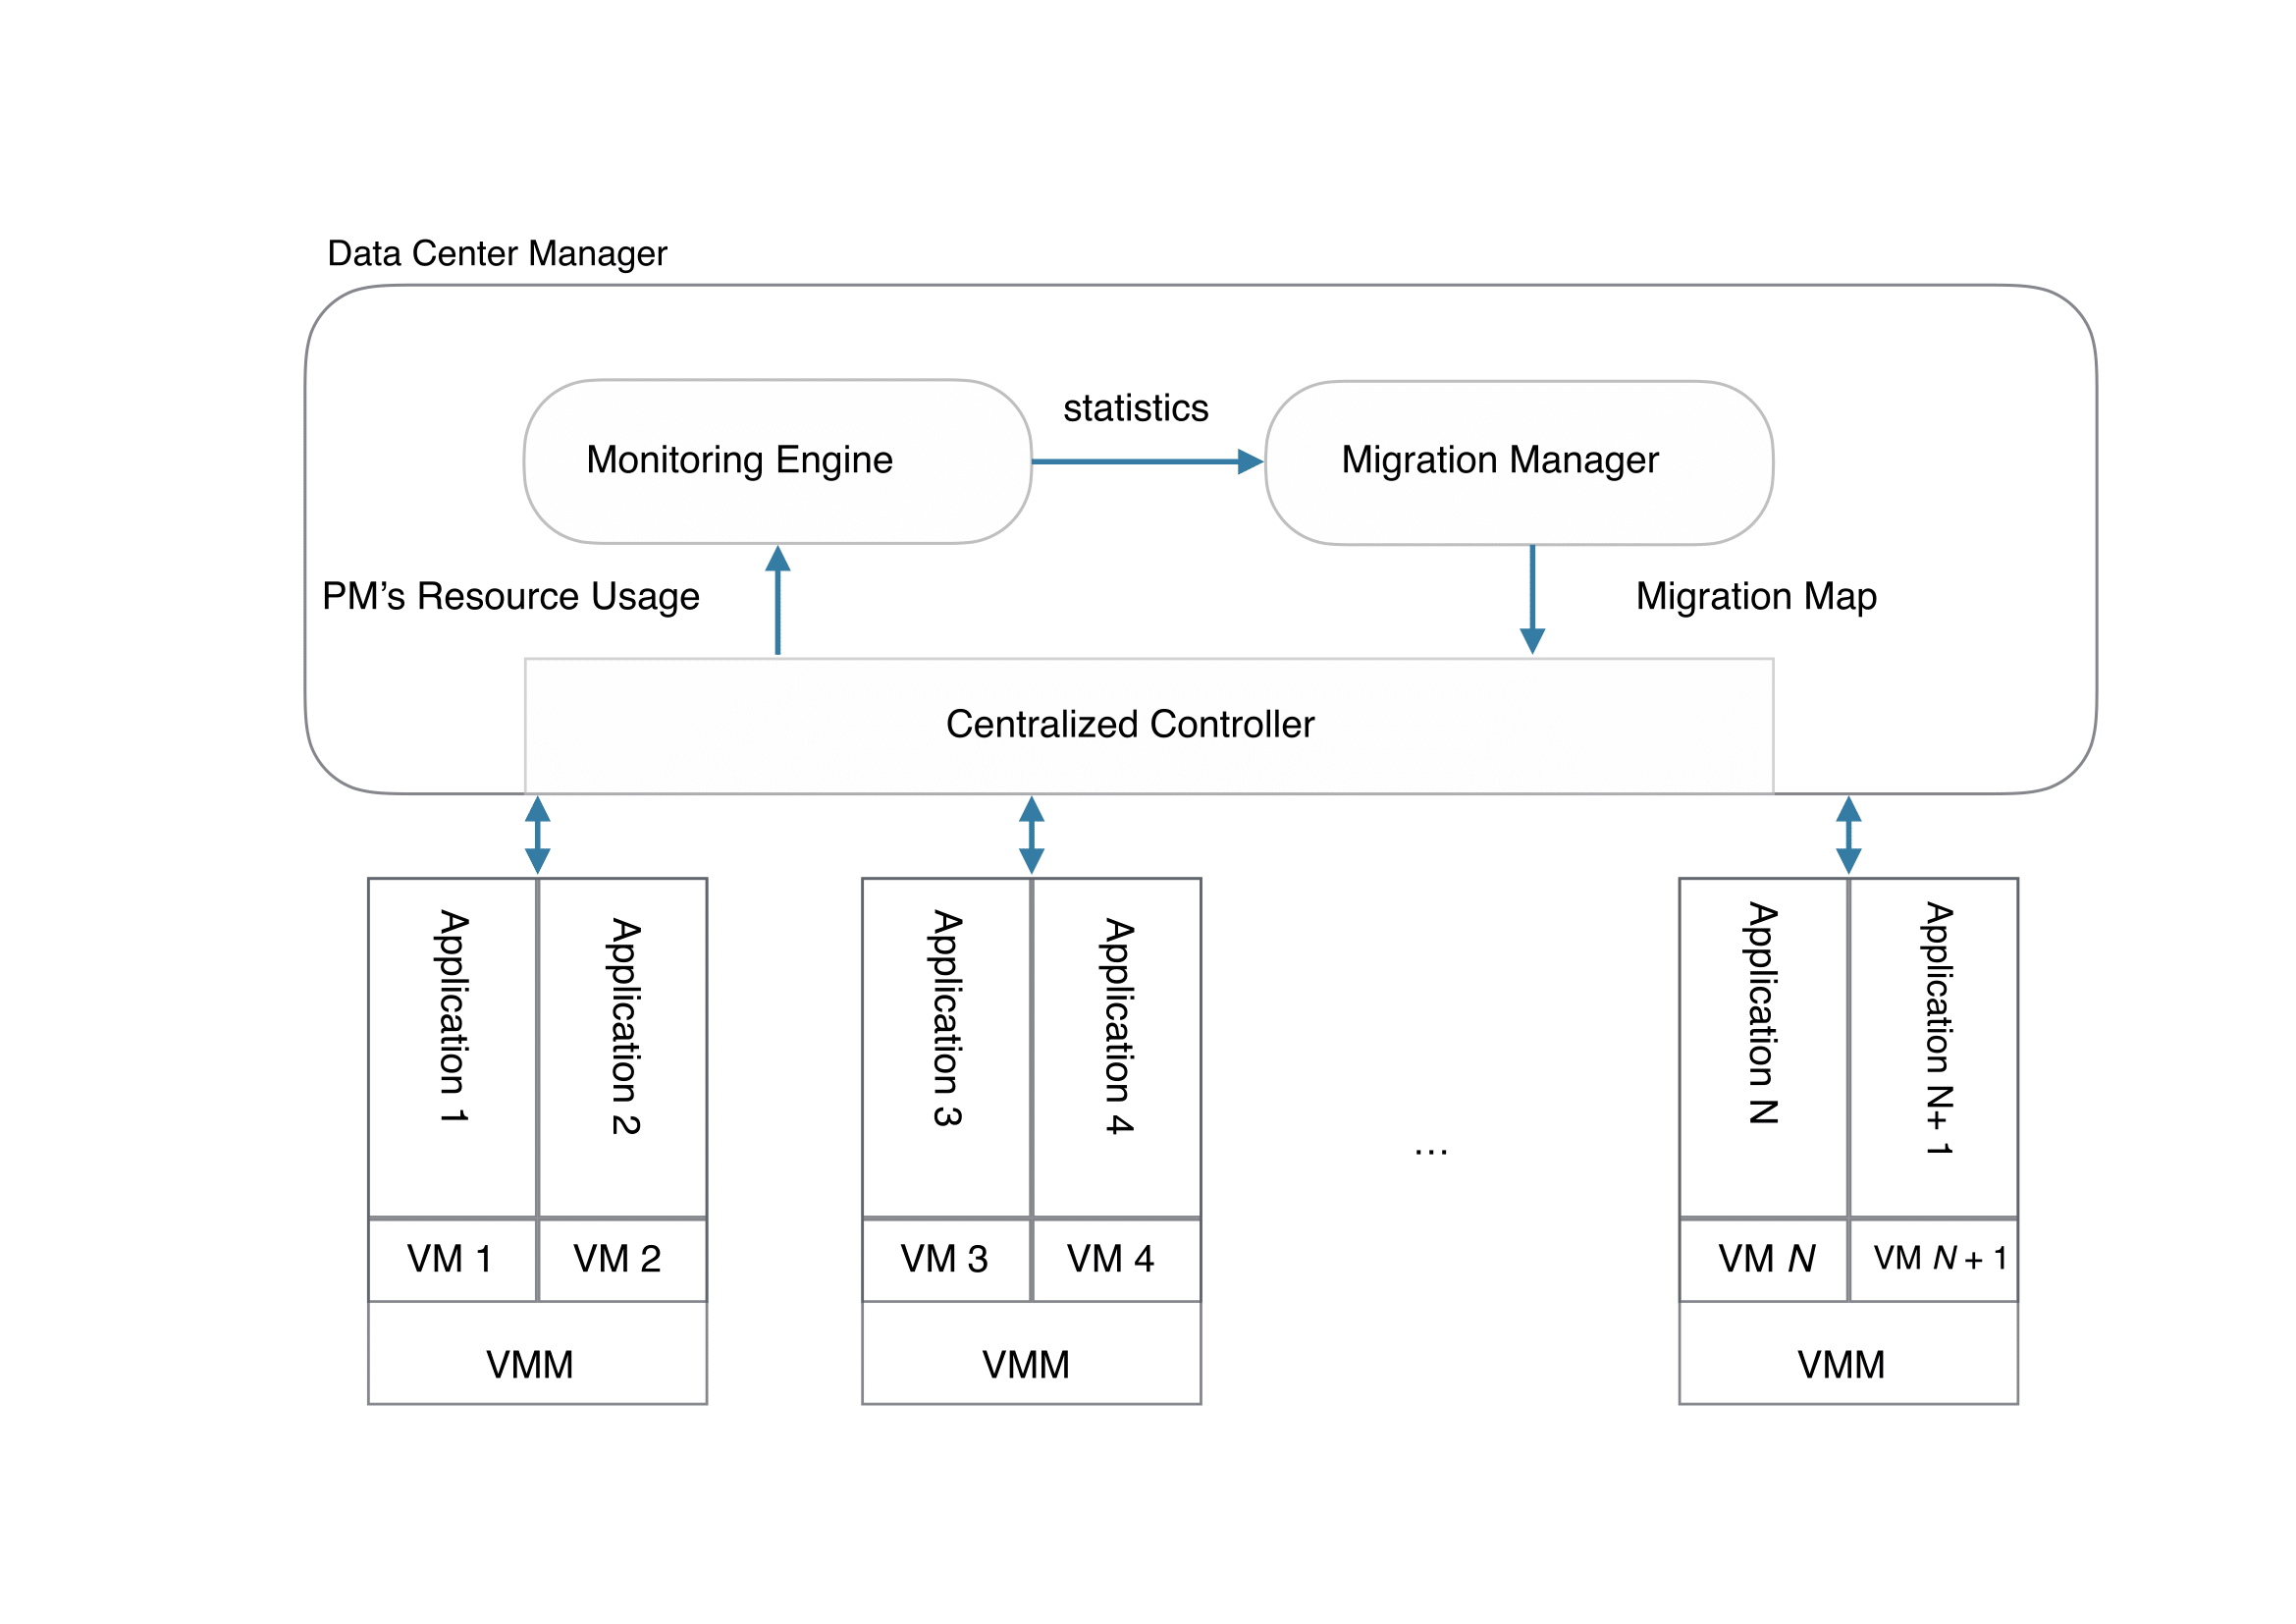
\includegraphics[width=1.0\textwidth]{pics/dataCenter-1.png}
% 	\caption{A datacenter management model \cite{Varasteh:2015fu}}
% 	\label{fig:arch}
% \end{figure}

% The taxonomy of server consolidation has not reach an agreement. In Verma's work \cite{Verma:2009wi}, they categorize it into three groups: static, semi-static and dynamic consolidation. In static consolidation, applications are placed on PM without any further movement. Semi-static refers to periodical adjustment. Dynamic consolidation is still applied on a set of VMs in response to their workload variations.









% A dynamic server consolidation approach
% can usually be decomposed into a series of steps, 
% reflecting the process required to produce a solution \cite{}. 
% These steps are shown in Figure \ref{} and discussed below:
% \begin{enumerate}
% 	\item When to migrate. Dynamic migration occurs on two scenarios: migrating VMs from overloaded server; and item migrating VMs from underloaded server.
% 	\item Which VMs to migrate.  After deciding to migrate a VM from a server, the next step is 
% 	to make a decision of which VM to migrate.
% 	\item Where to migrate the VMs. The key step is to determine where to allocate a VM which leads to global optimization.
% \end{enumerate}


% \subsection*{A Comparison between CaaS and IaaS based Cloud model}
% From a computing system design point of view, we believe service allocation and VM Placement
% are closely related and should be considered as a single allocation task.
% \subsection*{Service Allocation}
% Service allocation refers to the process of mapping a Web service on a certain type of VM.
% It is conducted by Cloud customers (e.g Web service providers) or Cloud brokers deligated by a 
% Cloud customer.
% The resource mapping involve with two steps, 
% resource demand profiling \cite{} and VM selection \cite{}. 
% Resource demand profiling is an estimation of the workload of a service. 
% Because the web application has dynamic workload over time \cite{}, 
% service providers or cloud brokers normally would like to estimate the future workload so that they 
% can choose how much resources to rent in order to guarantee the 
% Service Level Agreements (SLAs)  \cite{} to end customers. In this step, historical statistics
% are often used and based on its peak workload estimation, service providers often
% rent resources more than they need. Since the peak workload only accounts for a small portion
% of its total operation time, intelligent strategies are applied to tackle the over-provisioning and 
% under-provisioning problems.

% Public Cloud providers often provide various configurations of VM, 
% often refered to as VM types or instance types \cite{Li:2011ti}. 
% An instance type is defined as its resources such as memory size, number of processors and 
% CPU frequency. 

% Previous research focus on how to rent an appropriate amount of resources so that it minimize the 
% service providers' costs.

% Ref \cite{Candeia:2010wt} considers e-Science applications with bag-of-tasks (BoT) model. It
% aims at executing a bag of independent tasks with the least amount of Cloud resources before
% a deadline.
% Unlike a service allocation problem, where service is permanantly deployed in a reserved VM, 
% they consider an on-demand VM allocation. 
% That means, when a bag of tasks comes, the system
% dynamically assign a set of VM to execute these tasks. 
% It evaluates four heuristic algorithms and 
% concludes that a greedy-based approach achieves the best result.

% Li et al \cite{Li:2011ti} consider a dynamic cloud scheduling problem 
% from Cloud brokers' perspective. It considers scenarios such as Cloud provider changing its offer 
% (e.g changing of pricing schemes or VM types) and service performance changing, 
% a cloud broker needs to adjust the VMs allocation across multiple Cloud providers. 
% This work proposes a model which maximize a Cloud consumers' profit by adjusting VMs across
% multiple Clouds. Their model does not consider a Cloud provider's profit.

% Wang and Xia \cite{Wang:2016ui} propose a MIP formulation for energy-aware VM placement in Cloud.
% The major difference between their work and previous work is that they use a non-linear energy model \cite{Gandhi:2009wp}.  Based on this model, they consider two resources CPU and memory. In order to solve the non-linear problem, they propose a linearization method which uses piecewise linear function to approximate the non-linear objective function. In the end, they uses a relaxation method to relax the integer linear programming problem into continuous and apply a rounding function to obtain a near-optimal solution. In summary, the energy model is the key objective in consolidation problem. With different models, the applied algorithm can be very different. However, EC approaches can deal with both linear and non-linear problem without any changes. That is an obvious advantage. 

% Virtualization technology was first developed in IBM System/360 in 1960s 
% targeting a finer granularity resource management. 
% It partitions a physical machine into separated resources 
% called virtual machine (VM) which can be allocated 
% and moved from one server to another. 
% This flexibility not only allows resources to be managed in a dynamic manner, 
% but also enables server consolidation.

% In a Cloud datacenter, server consolidation is used as technique to combat \emph{server sprawl}.
% Server sprawl refers to the low utilization of physical servers. The main cause for server sprawl is
% the requirement of running applications in isolation \cite{Vogels:2008bg}. 
% That is, an application is deployed in one or more servers which 
% offer much more resources than it needs. 
% With full virtualization \cite{}, a server's physical resources including CPUs, memory, and I/O devices
% are divided into finer granularity level of resources.
% Virtual machines offer different sizes of resources that 
% can be choosed to satisfy different demands from applications. 

% \subsection*{An Overview of Evolutionary Computation}


% \subsection*{Initial Placement}

% \section*{Container-based VM Multiplexing}
% Container has been introduced back in the 1980s' \cite{}. The recent development of container
% allows only one process running in a container; this is revolutionary invention is called application
% container. It plays an important role in Cloud computing since it is lightweighted, easier to configure
% and enable finer adjustment than the VM-based resource management.


% \begin{figure}
% 	\centering
% 	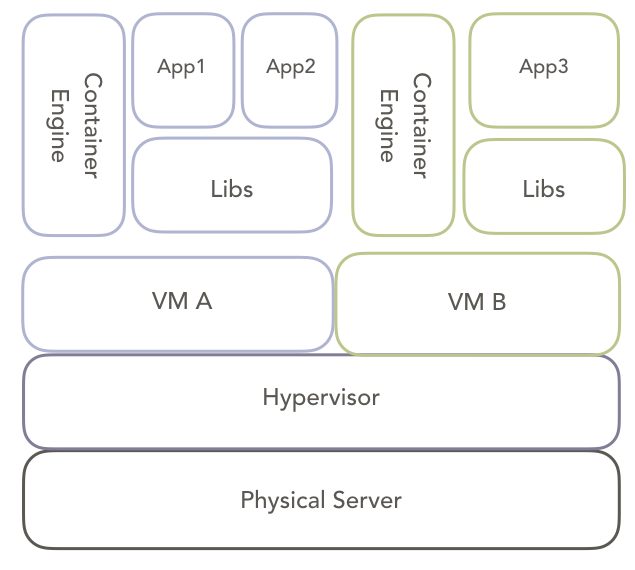
\includegraphics[width=0.6\textwidth]{pics/container.png}
% 	\caption{A Container as a Service Deployment Model}
% 	\label{fig:container}
% \end{figure}

% % % % % \section*{Dynamic VM Placement}
% % % % The traditional dynamic VM placement approaches can be categorized into three groups: Heuristic
% % % based approaches, deterministic approaches and dyanmic techniques with load prediction.

% % However, we believe the dynamic VM placement problem is highly dependent on an overall workload

% \section*{Large scale VM Placement}
% If you are writing an MSc or PhD thesis you should \emph{not} be using this style. Instead use \verb=vuwthesis=, which is based on the book style, and conforms to the VUW thesis rules. The thesis style is rather different from the project report style. 

% This document is formatted using a local (to ECS and MSOR at VUW) style file. When you write your project report you should be very careful when changing the beginning. The document class settings should read:

% \begin{verbatim}
% \documentclass[11pt
%               , a4paper
%               , twoside
%               , openright
%               ]{report}
% \end{verbatim}
% The options to the document class specify that:
% \begin{itemize}
% \item 11pt font is to be used for the main body text,
% \item  we will print on A4 paper, 
% \item we will use duplex (two-sided) printing,
% \item we want chapters to start on a right-hand page. 
% \end{itemize}

% The opitons you supply to the  \texttt{vuwproject} style will depend upon
% what you are using the style for.

% \subsection{Specifying the details}
% The \texttt{vuwproject} style sets up the front page properly, and provides various commands allowing you to specify the author, title, supervisor or supervisors, the school from which the report is being submitted and the degree that the report is being submitted for. The style has deliberately been designed to do as little as possible. This means that your document can easily be re-formatted as a technical report, or for submission to a conference or journal by using the appropriate style.

% It is also possible to use the style to easily produce documents on a
% stand-alone computer where your \LaTeX installtion might not have all
% of the  files and fonts available to machines within ECS or MSOR.

% Most of the options to the \texttt{vuwproject} style are currently a simple
% choice and there's a default that will make it obvious if you do not make
% a choice.

% Use one of the following options to use fonts available on ECS/MSOR machines
% or to use images that imitate them (assumes you have copies of the images)
% \begin{itemize}
% \item \verb+font+
% \item \verb+image+
% \end{itemize}

% Use one of the following options to set the school,
% \begin{itemize}
% \item \verb+ecs+
% \item \verb+msor+
% \end{itemize}

% Use one of the following options to choose a pre-defined degree,
% \begin{itemize}
% \item \verb+bschonscomp+
% \item \verb+mcompsci+
% \end{itemize}

% or use this command to use an explicit degree or diploma name
% \begin{itemize}
% \item \verb+\otherdegree{DEGREE OR DIPLOMA NAME}+
% \end{itemize}

% So, for example, to submit a report for the Master of Comp Sci degree, which
% the style knows about, from within ECS, using the images, you'ld ensure the
%  \texttt{vuwproject} line options looked like:

% \begin{verbatim}
% \usepackage[image,ecs,mcompsci]{vuwproject}
% \end{verbatim}

% whereas for a degree from within MSOR, when creating the final version on
% an ECS or MSOR machine where you have access to the fonts, you would use
% these options

% \begin{verbatim}
% \usepackage[font,msor]{vuwproject}
% \end{verbatim}


% and add the other degree's name using this command 

% \begin{verbatim}
% \otherdegree{DEGREE OR DIPLOMA NAME}
% \end{verbatim}

% To specify the supervisor or supervisors use either of the following commands in the preamble.
% \begin{itemize}
% \item \verb+\supervisor{The Supervisor}+
% \item \verb+\supervisors{Super 1 and Super 2}+
% \end{itemize}

% If you fail to set any degree or supervisor, or the school, then the front page will report this.

% The \texttt{vuwproject} style also sets the default font to be Palatino, using the \texttt{mathpazo} package. Palatino is one of VUW's `offical' fonts, and is the font used for the heading on the front page. The \texttt{mathpazo} package also typesets maths in a style which suits Palatino. 

% \section{Copying the style}
% If you want to write your project report away from VUW you will need to make your own copy of the \texttt{vuwproject} style.

% You can find out where the original lives by reading the messages that \LaTeX\ prints when it is run.

% Alternatively, you can down load a copy of the  \texttt{vuwproject} style from
% the ECS webpages.

% Any changes made to your own copy of the \texttt{vuwproject} style will not be reflected in the original, and \textit{vice versa}. Hence it makes sense to leave this as it is, and use a local style file for your own definitions.   
